\subsection{Datos Generales de la Empresa}

\subsubsection{Reseña histórica de la empresa}
J\&P Periféricos S.A.C. es una empresa peruana del sector informático que inició sus operaciones el 1 de octubre del año 2011. Su propósito es brindar soluciones informáticas a empresas cuyas necesidades son la mejora de sus procesos internos. Asimismo, ofrece la venta de productos tecnológicos tanto a personas naturales como empresas.

Con el paso de los años, J\&P Periféricos fue logrando consolidar su presencia en el sector y especializando sus soluciones de acuerdo a las necesidades de sus clientes. Además, ha ampliado el alcance de sus servicios, dando mantenimiento y soporte técnico continuo con el fin de alcanzar una mayor credibilidad y mejorar la relación con sus clientes.

\subsubsection{Quiénes Somos}
J\&P Periféricos S.A.C. es una empresa peruana en el rubro de la informática que brinda soluciones integrales informáticas tales como el mantenimiento informático, venta de productos tecnológicos, desarrollo de páginas web, redes y comunicaciones, empleando tecnología actual para una mejor eficiencia y rapidez en sus procesos.

\subsubsection{Razón Social}

{
    \centering
    \renewcommand{\arraystretch}{1.35}
    \setlength{\tabcolsep}{4pt}
    \begin{tabular}{
        @{}
        p{2.8cm}
        p{4.8cm}
        @{\hspace{0.2cm}}
        p{2.8cm}
        p{4.8cm}
        @{}
    }
        \textbf{Empresa} & 
        J\&P Periféricos S.A.C. & 
        \textbf{Empresario} 
        & Julio Flores Vicuña 
        \\[2pt]
        
        \textbf{RUC} &
        20545122520 &
        \textbf{Rubro} &
        Soluciones Informáticas
        \\[5pt]
        
        \textbf{Distrito} &
        Cercado de Lima & 
        \textbf{Dirección} &
        {\raggedright Jr. Emilio Fernández 160 Dpto. 1804\par}
        \\
    \end{tabular}
    \par
}
\clearpage
\subsubsection{Logo de la Empresa}

\begin{center}
    \vspace{0.1cm}
    %  Identificador y título en formato APA 7
    \refstepcounter{figure}
    \label{fig:logo_empresa}

    \addcontentsline{lof}{figure}{%
        Figura~\thefigure. Logotipo institucional de
        J\&P Periféricos S.A.C.}

    {\bfseries Figura~\thefigure}\par\vspace{0.1cm}
    {\itshape Logotipo institucional de J\&P Periféricos S.A.C.}\par
    \vspace{0.25cm}

    % Imagen del logo
    
\includegraphics[width=0.52\linewidth]{images/J&P_Logo.png}\par
    \vspace{0.25cm}

    % Nota explicativa alineada al ancho de la imagen
    \begin{minipage}{0.52\linewidth}
        \small
        \textit{Nota.} Gráfico representativo del logotipo corporativo de la empresa.
    \end{minipage}
\end{center}

\subsubsection{Ubicación de la Empresa}

La sede de \textbf{J\&P Periféricos S.A.C.} se encuentra ubicada en el departamento Concepto Urbano Plus, Calle Emilio Fernández 160, Dpto. 1804, distrito de Cercado de Lima (Código Postal 15046). Como referencia de acceso principal, el inmueble se ubica a la altura de la cuadra 8 de la Avenida Arequipa.

\begin{center}
    % Título formato APA 7 (Recto / Sin cursiva)
    \refstepcounter{figure}
    \label{fig:ubicacion_empresa}
    \addcontentsline{lof}{figure}{%
        Figura~\thefigure.
        Localización y vías de acceso de la empresa}

    {\bfseries Figura~\thefigure}\par
    {\itshape Localización y vías de acceso de la empresa}\par
    \vspace{0.20cm}

    % Imagen con borde gris tenue
    {\color{gray!60}\setlength{\fboxsep}{0pt}\setlength{\fboxrule}{0.6pt}%
    \fbox{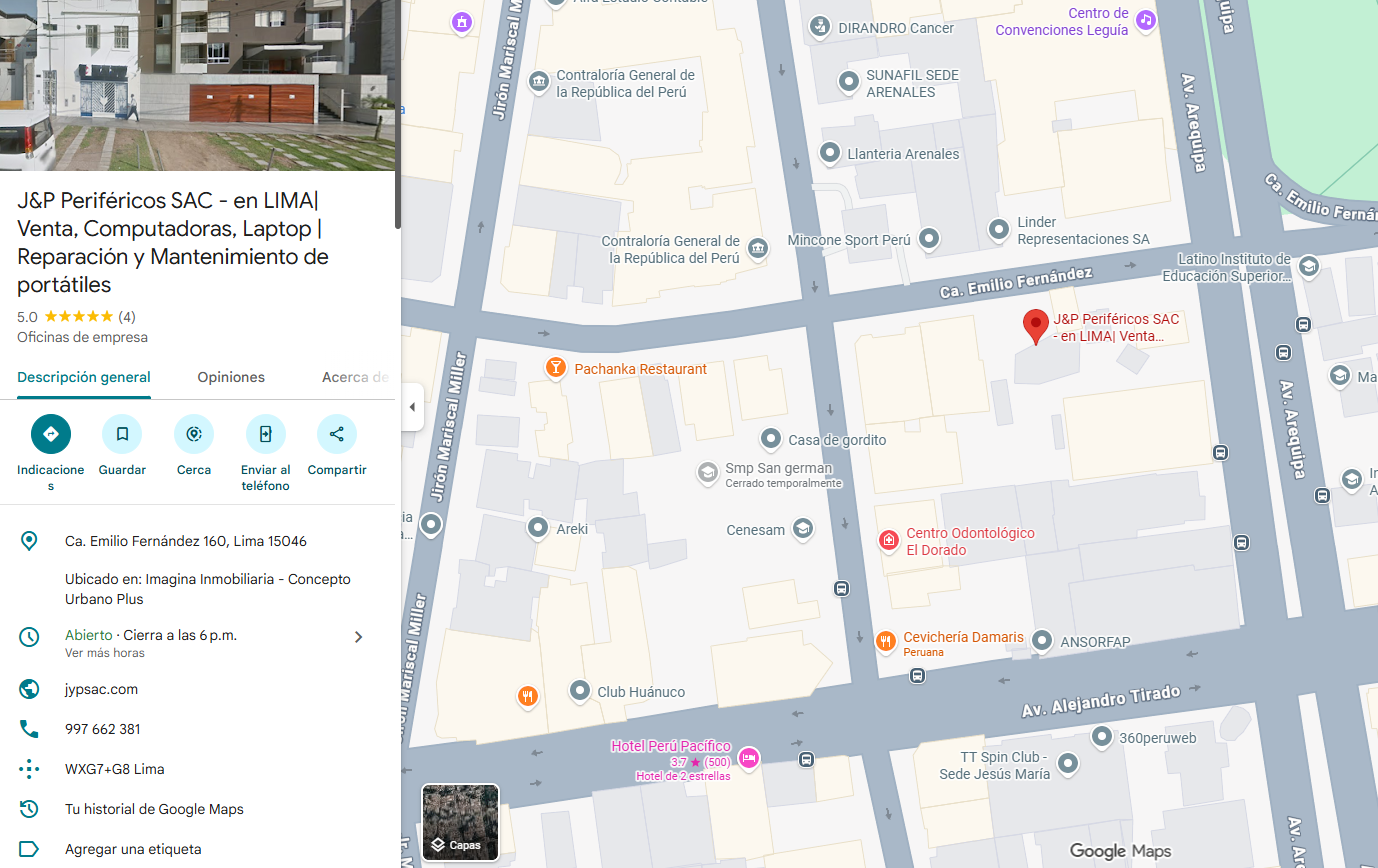
\includegraphics[width=0.90\linewidth, height=6cm, keepaspectratio=false]{images/ubicacion_empresa.png}}}\par
    \vspace{0.25cm}

    % Nota APA 7 alineada al ancho de 0.90
    \begin{minipage}{0.90\linewidth}
        \small
        \textit{Nota.} Ubicación geográfica y mapa vial de la sede central. Adaptado de Google Maps.
    \end{minipage}
\end{center}
